\documentclass[border=10pt]{standalone}

%Drawing
\usepackage{tikz}
\usetikzlibrary{intersections}
\usetikzlibrary{calc}


\newcommand{\drawRectangle}[2]{
   	\draw[fill=blue, opacity=0.2] ($(#1,#2) - (0.5,0.5)$) rectangle ($(#1,#2) + (0.5,0.5)$) ;   
}

\begin{document}
	
	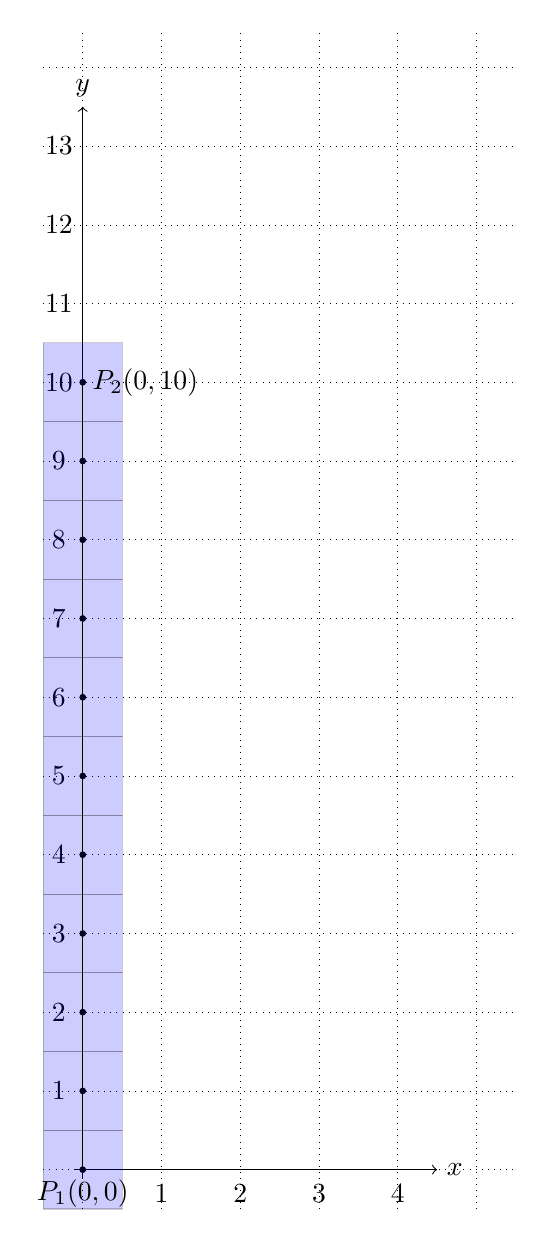
\begin{tikzpicture}
%%%%%%%%%%%%%%%%%%	

%Grid
\draw[very thin, dotted] (-0.5,-0.5) grid (5.5,14.5);
	\foreach \i in {1,...,4}
	{
		\node at (\i,-2ex) {\i};	
%		\node at (-2ex,\i) {\i};				
	}
	\foreach \i in {1,...,13}
	{
		\node at (-2ex,\i) {\i};				
	}
%Draw axes
    \draw[->] (-0.1, 0) -- (4.5, 0) node[right] {$x$};
\draw[->] (0, -0.1) -- (0, 13.5) node[above] {$y$};
    
    (0,0),(0,1),(0,2),…,(0,10)
% Plot points
    \filldraw[black] (0, 0) circle (1pt) ;
	\filldraw[black] (0, 1) circle (1pt) ;
	\filldraw[black] (0, 2) circle (1pt) ;
	\filldraw[black] (0, 3) circle (1pt) ;
	\filldraw[black] (0, 4) circle (1pt) ;
	\filldraw[black] (0, 5) circle (1pt) ;
	\filldraw[black] (0, 6) circle (1pt) ;
	\filldraw[black] (0, 7) circle (1pt) ;
	\filldraw[black] (0, 8) circle (1pt) ;
	\filldraw[black] (0, 9) circle (1pt) ;			
	\filldraw[black] (0, 10) circle (1pt) ;				

%	\fill[blue, opacity=0.2] (1,1) rectangle (2,2) ; 
\drawRectangle{0}{0}   
\drawRectangle{0}{1}
\drawRectangle{0}{2}   
\drawRectangle{0}{3}   
\drawRectangle{0}{4}   
\drawRectangle{0}{5}   
\drawRectangle{0}{6}   
\drawRectangle{0}{7}   
\drawRectangle{0}{8}   
\drawRectangle{0}{9}   
\drawRectangle{0}{10}   
% Connect points with a line
    \draw[very thin] (0, 0) -- (0, 10);
    \draw[dashed, very thin] (0, 0) -- (0, 10);


    \node[below] at (0,0) {$P_1(0,0)$};
    \node[right] at (0,10) {$P_2(0,10)$};
\end{tikzpicture}

\end{document}



